\documentclass[conference,11pt]{IEEEtran}
\usepackage{amsmath,amssymb,amsthm,graphicx,booktabs,cite,url,array}
\newtheorem{proposition}{Proposition}
\newtheorem{theorem}{Theorem}
\theoremstyle{definition}\newtheorem{remark}{Remark}
\newcommand{\Gm}{\Gamma}
\begin{document}
\title{Robust Carbon-Aware Workflow Scheduling\\ under Budgeted Forecast Uncertainty}
\author{\IEEEauthorblockN{Ishita Singh, Aayushi Uikey, Jahnavi Yadav}
\IEEEauthorblockA{Department of Computer Science and Engineering, RGIPT\\ Advanced Algorithm}}
\maketitle

\begin{abstract}
Data-centre workflows are DAGs of tasks with a deadline, and delaying flexible tasks to low-carbon hours reduces emissions. Existing carbon-aware schedulers treat the hourly carbon forecast as exact. We study scheduling when each slot's carbon intensity may deviate from its forecast by a bounded amount, at most $\Gm$ slots deviate at once, and total power per slot is capped. We give (i) an exact worst-case cost and a dual linear form that yields a mixed-integer program (MILP) of almost the original size, (ii) a proof of strong NP-hardness by reduction from 3-Partition, (iii) an exact polynomial algorithm for a chain of tasks on one processor based on a threshold decomposition, and (iv) \textsc{RobSlack}, a threshold-cost construction with local search that never does worse than ASAP. On synthetic but calibrated data, \textsc{RobSlack} is within 1.3\% of the exact optimum on average on small instances. We also find that on large workflows a well-optimised nominal plan is already robust on average; budgeted-robust plans matter for short, concentrated workloads, where they remove rare days on which the forecast-optimal plan emits more than running immediately.
\end{abstract}
\begin{IEEEkeywords}
carbon-aware scheduling, robust optimisation, workflow scheduling, NP-hardness, uncertainty
\end{IEEEkeywords}

\section{Introduction}
Electricity carbon intensity (g\,CO$_2$/kWh) varies by hour, so identical work emits different amounts depending on when it runs. A workflow has precedence constraints and a deadline $D$; the gap between its earliest finish and $D$ is slack that can be used to shift work. The forecast, however, is only a forecast. A plan that chases the greenest-looking hour can be worst exactly when that hour is least reliable (Section~\ref{sec:model}, Table~\ref{tab:tiny}).

\textbf{Contributions.} We combine (a) a $\Gm$-budgeted uncertainty set on carbon intensity, (b) precedence-constrained workflows with a deadline, and (c) a per-slot power cap, and provide (d) an exact robust model, (e) hardness and a polynomial special case, (f) a heuristic that never regresses against ASAP, and (g) an evaluation including fixed plans versus re-planning. We claim the combination and the evidence, not priority.

\section{Related Work and What Is New}
\textbf{Carbon-aware workflow scheduling.} CaWoSched~\cite{cawo25} schedules a workflow whose task mapping and order are given, under a deadline and a known time-varying carbon profile. It is polynomial on one processor and NP-hard on two or more, and the authors propose 16 greedy-plus-local-search heuristics, a baseline and an ILP. A later study extends the setting to joint mapping and scheduling on real hourly carbon-intensity data~\cite{cawo26}. \textbf{Precedence-aware clusters.} PCAPS~\cite{pcaps25} schedules DAG jobs on data-processing clusters online; the carbon signal is unknown but assumed to lie between known bounds, and evaluation is empirical. \textbf{Robust optimisation.} Our uncertainty model follows the budget-of-uncertainty framework of Bertsimas and Sim~\cite{bs04}; our baseline list scheduler follows the HEFT rank ordering~\cite{heft02}.

\textbf{What we add.} The works above treat the forecast as exact or only loosely bounded, and none has a per-slot power cap together with an error budget. We contribute a $\Gamma$-budgeted per-slot error model combined with precedence, deadline and a power cap; an exact dual MILP; a robust polynomial algorithm for a fixed-order chain, the $\Gamma$-robust analogue of the one-processor result; hardness for free ordering; and a heuristic with a no-regression guarantee evaluated against exact optima and with fixed versus re-planned schedules. Our hardness result concerns free task ordering and is therefore different from the fixed-order NP-hardness for two or more processors in~\cite{cawo25}. In our searches we found no paper with this exact combination, but the review is not complete and the closest theory work on $\Gamma$-robust scheduling with start-time-dependent costs must still be read carefully; we claim the combination and the evidence, not priority.

\section{Model}\label{sec:model}
A task $v$ has duration $d_v$ slots, power $p_v$ and a fixed processor. Precedence $(u,v)$ requires $u$ to finish before $v$ starts. Slots $0,\dots,D-1$ have length $h$ hours. A schedule $S$ assigns a start slot to every task. It is \emph{feasible} if tasks end by $D$, precedence holds, each processor runs one task at a time, and total power $P_S(t)=\sum_{v\text{ running at }t}p_v$ is at most the cap $\kappa$ in every slot.

Forecast carbon is $c_t$, the maximum error is $e_t$, and $\Gm$ is the budget. The nominal cost is $N(S)=h\sum_t c_tP_S(t)$. An adversary raises at most $\Gm$ slots to their maximum error (a fractional part of $\Gm$ applies to the next-largest slot). The worst-case cost is
\begin{equation}
W(S)=N(S)+h\,R_\Gm(S),\quad R_\Gm(S)=\sum_{\text{$\Gm$ largest}} e_tP_S(t).
\end{equation}
Because the error term uses the \emph{total} power of a slot, tasks cannot be priced independently; this is what makes the DAG version harder than the single-job version.

\begin{table}[t]\centering\caption{Tiny example: one task, 2 slots, 1\,kW, $\Gm=1$. Forecast $200,300,80,250,150$; max error $10,20,200,20,20$.}\label{tab:tiny}
\begin{tabular}{lcc}\toprule Start & Forecast cost & Worst-case cost\\\midrule
0 (ASAP) & 500 & 520\\ 1 & 380 & 580\\ 2 (nominal-optimal) & 330 & 530\\ 3 (robust-optimal) & 400 & 420\\\bottomrule\end{tabular}\end{table}

\section{Theory}\label{sec:theory}
Throughout, $P_S(t)$ is the total power in slot $t$, $x_t=e_tP_S(t)$ is the error exposure of slot $t$, and $R_\Gamma(S)=\sum_{\Gamma\text{ largest}}x_t$, so that $W(S)=N(S)+h\,R_\Gamma(S)$.

\subsection{Exact linear form}
\begin{proposition}[Dual form of the adversary]\label{prop:dual}
For $x\ge0$ and $\Gamma\ge0$,
\begin{equation}
\max_{\substack{u\in[0,1]^T\\ \sum_tu_t\le\Gamma}}\sum_t x_tu_t \;=\; \min_{\theta\ge0}\;\Big[\Gamma\theta+\sum_t\max(x_t-\theta,0)\Big].\label{eq:dual}
\end{equation}
\end{proposition}
\begin{proof}
The left side is a linear program in $u$. Let $\theta$ be the dual variable of the budget constraint and $q_t\ge0$ the dual of $u_t\le1$; strong LP duality gives the right side with $q_t=\max(x_t-\theta,0)$.
\end{proof}
Hence the exact robust problem is the MILP
\begin{align}
\min\;& h\Big[\sum_tc_tP(t)+\Gamma\theta+\sum_tq_t\Big]\label{eq:obj}\\
\text{s.t.}\;& q_t\ge e_tP(t)-\theta,\quad q_t,\theta\ge0,\label{eq:rob}\\
& \text{start, precedence, processor and cap constraints},\nonumber
\end{align}
with time-indexed start variables $z_{v,s}\in\{0,1\}$. It has only $T+1$ more continuous variables than the nominal model.

\subsection{Structural properties}
\begin{proposition}[Monotone and concave in $\Gamma$]\label{prop:conc}
For fixed $S$, $R_\Gamma(S)$ is nondecreasing and concave in $\Gamma$. Hence $V(\Gamma)=\min_SW(S)$, a minimum of concave functions, is nondecreasing and concave, and $N(S)\le W(S)\le N(S)+h\sum_tx_t$.
\end{proposition}
\begin{proposition}[Price of robustness]\label{prop:price}
Let $S^0$ minimise $N$ and $S^R$ minimise $W$. Then
\begin{multline}
0\le N(S^R)-N(S^0)\\\le h\big[R_\Gamma(S^0)-R_\Gamma(S^R)\big]\le h\,R_\Gamma(S^0),
\end{multline}
and $W(S^R)\le W(\mathrm{ASAP})$.
\end{proposition}
\begin{proof}
$W(S^R)\le W(S^0)$ gives $N(S^R)+hR_\Gamma(S^R)\le N(S^0)+hR_\Gamma(S^0)$, and $N(S^R)\ge N(S^0)$ by optimality of $S^0$. ASAP is feasible, so $W(S^R)\le W(\mathrm{ASAP})$.
\end{proof}

\subsection{Complexity}
\begin{theorem}[Strong NP-hardness]\label{thm:hard}
Minimising $W$ is strongly NP-hard, even with one processor, no precedence, $\Gamma=0$ and unit power.
\end{theorem}
\begin{proof}
Reduce from 3-Partition~\cite{gj79}: integers $a_1,\dots,a_{3m}$ with $B/4<a_i<B/2$ and $\sum a_i=mB$.
\begin{enumerate}
\item Create a task of duration $a_i$ for each integer; set $D=mB+m-1$.
\item Slots $j(B+1)-1$ for $j=1,\dots,m-1$ get carbon 1; all other slots get carbon 0.
\item Total task length equals the number of zero-carbon slots, so cost 0 is attainable iff every task lies inside one of the $m$ green windows of length $B$ and the windows are filled exactly.
\item The size bounds force exactly three tasks per window, each window summing to $B$: a 3-partition.
\end{enumerate}
$D$ is polynomial in the unary size of the input, so the hardness is strong.
\end{proof}

\subsection{Exact algorithm for a chain}
\begin{theorem}[Fixed-order chain on one processor]\label{thm:chain}
For tasks in a fixed order on one processor, $\min_SW(S)$ is computable in $O(q\,n\,D^2)$ time, where $q$ is the number of distinct powers.
\end{theorem}
\begin{proof}
\emph{Step 1 (finite $\theta$ set).} For fixed $S$, $F(S,\theta)=\Gamma\theta+\sum_t\max(x_t-\theta,0)$ is convex piecewise linear in $\theta$ with breakpoints in $\{e_tp_v\}$ and slope $\ge0$ for large $\theta$, so its minimum over $\theta\ge0$ lies in $\Theta=\{0\}\cup\{e_tp_v\}$, with $|\Theta|\le qD+1$.\\
\emph{Step 2 (exchange).} $\min_S\min_\theta=\min_{\theta\in\Theta}\min_S$.\\
\emph{Step 3 (separability).} On one processor $P(t)$ is the power of the single running task, so for fixed $\theta$ the cost is a sum of independent per-task, per-start costs $c_tp_v+\max(e_tp_v-\theta,0)$; the cap only removes starts.\\
\emph{Step 4 (DP).} A dynamic programme over the task order solves each $\theta$ in $O(nD)$.
\end{proof}
\begin{remark}
The result does not extend to general single-processor DAGs, which contain the hard case of Theorem~\ref{thm:hard}.
\end{remark}

\subsection{Safety of the heuristic}
\begin{proposition}[RobSlack safety]\label{prop:safe}
\textsc{RobSlack} returns a feasible schedule with $W\le W(\mathrm{ASAP})$.
\end{proposition}
\begin{proof}
ASAP is always a starting candidate and every local-search move preserves feasibility and does not increase $W$. We prove no approximation ratio.
\end{proof}

\subsection{Numerical verification}
\begin{table}[t]\centering\caption{Numerical checks of the theory.}\label{tab:checks}
\footnotesize\setlength{\tabcolsep}{3pt}
\begin{tabular}{p{0.52\columnwidth}p{0.38\columnwidth}}\toprule
Claim & Check\\\midrule
Closed form~\eqref{eq:dual} vs adversary enumeration & 200/200 cases\\
MILP~\eqref{eq:obj}--\eqref{eq:rob} vs exhaustive search & 58 instances, max diff $1.7\times10^{-10}$\\
$V(\Gamma)$ nondecreasing, concave & 20/20 instances\\
3-Partition reduction vs solver & 200/200 (158 yes, 42 no)\\
Chain DP vs exhaustive search & 59 instances, diff $2.7\times10^{-12}$\\
Chain DP vs MILP & 20 instances, rel.\ diff $\approx10^{-10}$\\
Chain DP runtime & $n=200$ in 0.45\,s\\\bottomrule\end{tabular}\end{table}

\section{Algorithms}
\textbf{Exact.} The time-indexed MILP above, solved with HiGHS (mean 1.4\,s on the small instances, all proven optimal).

\textbf{RobSlack.} For thresholds $\theta$ (quantiles of the $e_tp_v$ values, plus $\infty$), repeatedly place the ready task with least latest-start at the cheapest start under task costs $c_tp+\max(e_tp-\theta,0)$, accepting a start only if the remaining tasks can still be completed (ASAP check). Improve each candidate, including ASAP, by single-task move local search on the true $W$, then iterated local search with random two-task kicks; return the best.

\textbf{Baselines.} ASAP; HEFT-like upward-rank list scheduling; greedy cheapest-window (forecast-trusting, $\Gm=0$, no local search); nominal-optimal ($\Gm=0$ plan).

\section{Experimental Setup}
\textbf{Data (synthetic; to be replaced by real data).} Hourly actual intensity is a demand shape minus a solar dip scaled by a per-day cloudiness factor, minus a persistent wind process, plus noise. The day-ahead forecast uses mean cloudiness and wind persistence. The horizon is 48 slots. The per-slot $e_t$ is the 90th percentile of $|$actual$-$forecast$|$ on 60 training days (smoothed); evaluation uses 40 held-out days (mean absolute error about 52\,g/kWh, largest at midday).

\textbf{Workloads.} Random layered DAGs, durations 1--3 slots, power 1--4\,kW, 3--4 processors; deadline = ASAP makespan + slack. Small exact comparison: $n=8$--10. Large: $n=30$, three workflows. All schedules are re-verified by an independent checker, and emissions are evaluated on actual intensity.

\section{Results}
\begin{table}[t]\centering\caption{Gap to proven optimum of worst-case cost (E1, 40 small instances).}
\begin{tabular}{lcc}\toprule Method & Mean gap & Max gap\\\midrule
RobSlack & 1.3\% & 4.2\%\\ Greedy cheapest-window & 5.8\% & 19.0\%\\ Nominal-optimal & 5.8\% & 23.7\%\\ ASAP & 21.2\% & 34.0\%\\ HEFT-like & 21.9\% & 34.5\%\\\bottomrule\end{tabular}\end{table}
\textsc{RobSlack} matched the optimum exactly on only 1 of 40 instances; a separate 80-instance test with tight caps showed a worst gap near 30\%, so tight power caps are a known weakness.

\begin{table}[t]\centering\caption{Saving vs.\ ASAP on actual emissions, \% (days worse than ASAP, \%). 3 workflows $\times$ 40 days.}\label{tab:e2}
\footnotesize\setlength{\tabcolsep}{1.5pt}
\begin{tabular}{rcccccc}\toprule Slack & HEFT & Greedy & $\Gm$=0 & $\Gm$=2 & $\Gm$=4 & $\Gm$=8\\\midrule
2 & 1.6 (27) & 3.8 (31) & 6.5 (2.5) & 6.0 (2.5) & 5.3 (4.2) & 2.9 (14)\\
6 & 1.6 (27) & 1.7 (44) & 10.7 (0.8) & 9.8 (0) & 8.1 (0) & 5.9 (5.8)\\
12 & 1.6 (27) & 12.7 (18) & 18.1 (0) & 17.2 (0) & 16.4 (0) & 13.3 (2.5)\\
24 & 1.6 (27) & 11.7 (32) & 22.1 (1.7) & 21.2 (2.5) & 20.1 (2.5) & 17.9 (0.8)\\\bottomrule\end{tabular}\end{table}
Savings grow with slack (Fig.~\ref{fig:slack}). The forecast-trusting greedy method is fragile (worse than ASAP on 17--44\% of days). A well-optimised nominal plan is not fragile on average here, and robust plans pay for protection with lower mean savings (slack 12: 16.4\% at $\Gm=4$ vs.\ 18.1\% at $\Gm=0$; paired Wilcoxon tests significant). Planned worst-case bounds held on only 46\% ($\Gm=0$) to 87\% ($\Gm=8$) of cases, so the bound is a planning device, not a guarantee, under per-slot 90\% calibration.

\begin{figure}[t]\centering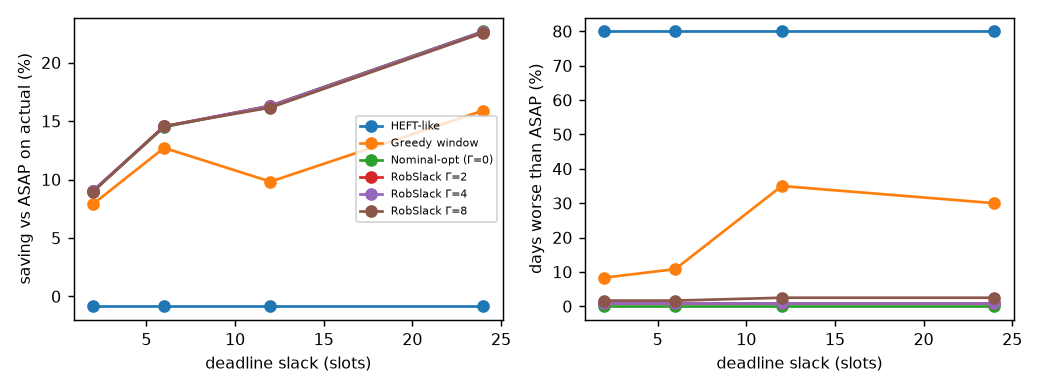
\includegraphics[width=\columnwidth]{fig_slack.png}\caption{Saving and fragility versus deadline slack.}\label{fig:slack}\end{figure}

\textbf{Where robustness pays (E7).} Using the exact chain algorithm over 40 test days: for one task with slack 16, the nominal plan saved 40.7\% but was worse than ASAP on 2.5\% of days (up to $1.07\times$); $\Gm\ge3$ saved 37.6\% with no such days (worst day $0.95\times$). For two tasks the nominal plan was worse than ASAP on 2.5\% of days (up to about $1.14\times$) and $\Gm=6$ reduced the worst case to about $1.0\times$ at about 3 points of saving. Caveat: 2.5\% of 40 days is one day, so evidence is thin.

\textbf{Price of robustness (E6, exact, $n=10$).} The mean optimal worst-case value rises from 8{,}938 ($\Gm=0$) to 14{,}174 ($\Gm=10$), concave and nondecreasing (Fig.~\ref{fig:price}); the forecast cost of the optimal plan rises 12.8\% by $\Gm=4$.

\begin{figure}[t]\centering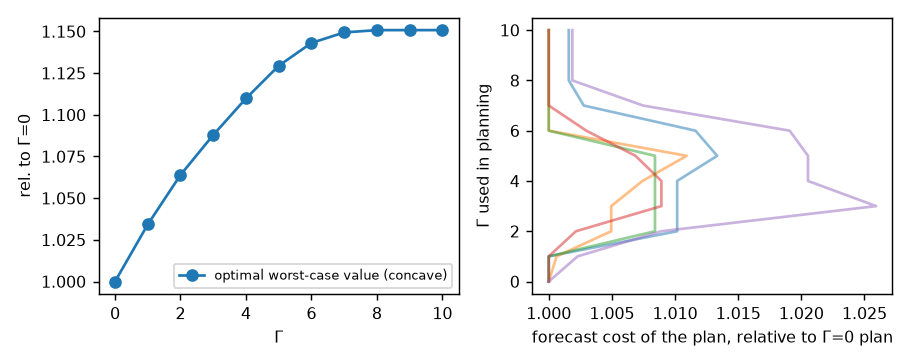
\includegraphics[width=\columnwidth]{fig_price.png}\caption{Price of robustness (exact, small instance).}\label{fig:price}\end{figure}

\textbf{Power cap (E3).} At slack 12, saving falls as the cap tightens (nominal / $\Gm=4$): no cap 14.6/13.4\%; $0.9\times$ peak 14.3/13.7\%; $0.75\times$ 13.0/12.0\%; $0.6\times$ 12.1/11.8\%; $0.5\times$ 5.3/5.1\% (Fig.~\ref{fig:cap}).

\begin{figure}[t]\centering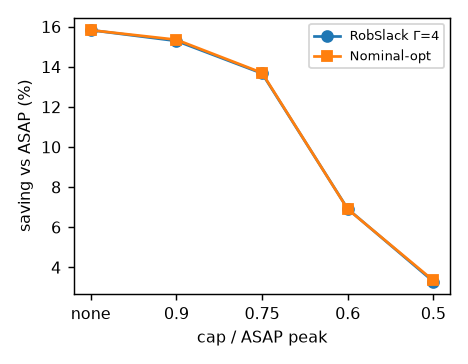
\includegraphics[width=0.6\columnwidth]{fig_cap.png}\caption{Effect of the power cap.}\label{fig:cap}\end{figure}

\textbf{Static vs.\ re-planning (E4).} Re-planning every 6 hours with revealed actuals and residual-decayed forecast updates: static nominal 14.2\%, static robust ($\Gm=4$) 13.1\%, re-planning nominal 14.8\%, re-planning robust 11.9\%. Nominal re-planning was best.

\section{Discussion and Limitations}
The hypothesis that forecast-optimal schedules are fragile is supported for forecast-trusting greedy heuristics and short concentrated workloads, but not for large well-optimised nominal plans on this synthetic data, where errors are roughly symmetric and average out over many slots. Real data may show biased, correlated errors; the honest message may be a regime map of when robustness helps. Limitations: synthetic data; fixed task-to-processor mapping; constant per-task power; uncertainty only in carbon; no approximation guarantee for \textsc{RobSlack} and a larger gap under tight caps; the chain algorithm needs one processor and a fixed order; small evaluation (40 days).

\section{Conclusion}
We gave an exact robust model, hardness, a polynomial special case and a safe heuristic for budgeted-robust carbon-aware workflow scheduling. Next: real forecast data, a complete literature review, a stronger heuristic under tight caps, and larger evaluations.

\begin{thebibliography}{6}
\bibitem{cawo25} D.~Schweisgut, A.~Benoit, Y.~Robert, and H.~Meyerhenke, ``Carbon-aware workflow scheduling with fixed mapping and deadline constraint,'' in \emph{Proc.\ 54th Int.\ Conf.\ Parallel Processing (ICPP '25)}, San Diego, CA, USA, 2025, doi:10.1145/3754598.3754673.
\bibitem{cawo26} D.~Schweisgut, A.~Benoit, Y.~Robert, and H.~Meyerhenke, ``Carbon-aware mapping and scheduling for deadline-constrained workflows,'' arXiv:2605.27652.
\bibitem{pcaps25} ``Carbon- and precedence-aware scheduling for data processing clusters,'' arXiv:2502.09717. [Authors to be added.]
\bibitem{bs04} D.~Bertsimas and M.~Sim, ``The price of robustness,'' \emph{Operations Research}, vol.~52, no.~1, pp.~35--53, 2004.
\bibitem{heft02} H.~Topcuoglu, S.~Hariri, and M.-Y.~Wu, ``Performance-effective and low-complexity task scheduling for heterogeneous computing,'' \emph{IEEE Trans.\ Parallel Distrib.\ Syst.}, vol.~13, no.~3, pp.~260--274, 2002.
\bibitem{gj79} M.~R.~Garey and D.~S.~Johnson, \emph{Computers and Intractability: A Guide to the Theory of NP-Completeness}. W.\,H.\ Freeman, 1979.
\end{thebibliography}
\end{document}
